\documentclass[../ClassicThesis.tex]{subfiles}
\begin{document}

% ************************************************
\chapter{Introduction}
\label{ch:introduction}
% ************************************************

\section{Fabrication Machines Enable Anyone to Bring Their Ideas to Life}
\label{sec:introduction}

% \note{maybe subdivide this package?}
% people are awesome -> ideas
% bringing ideas to live -> back in time -> difficult
% transition, changes now
% machines -> plug into your computer -> take over fabrication for you

% \note{people in general. no specific field or skillset.
% ideas always.}

People always had lots of creative ideas, regardless their
background or skill set. Though back in time it was
difficult realizing these due to the lack of specific
knowledge or tools. For example in the field of engineering,
when one has an idea how airplanes fly better
(Figure~\ref{fig:intro-ideas:plane}). There are ideas
concerning creative processes, like designing a fashion line
for shoes which offer correct fit to the feet of its wearer
(Figure~\ref{fig:intro-ideas:shoe}). Even in health care
broad ideas evolve. In 2013 Jake Evill presented
\name{Cortex}, a customizable plaster that is \enquote{fully
  ventilated, super light, shower friendly, hygienic,
  recyclable and
  stylish}\footnote{\url{http://www.evilldesign.com/cortex}}.
Cortex is shown in Figure~\ref{fig:intro-ideas:plaster}.

\begin{figure}[ht]
  \centering
  \begin{subfigure}[b]{\textwidth}
    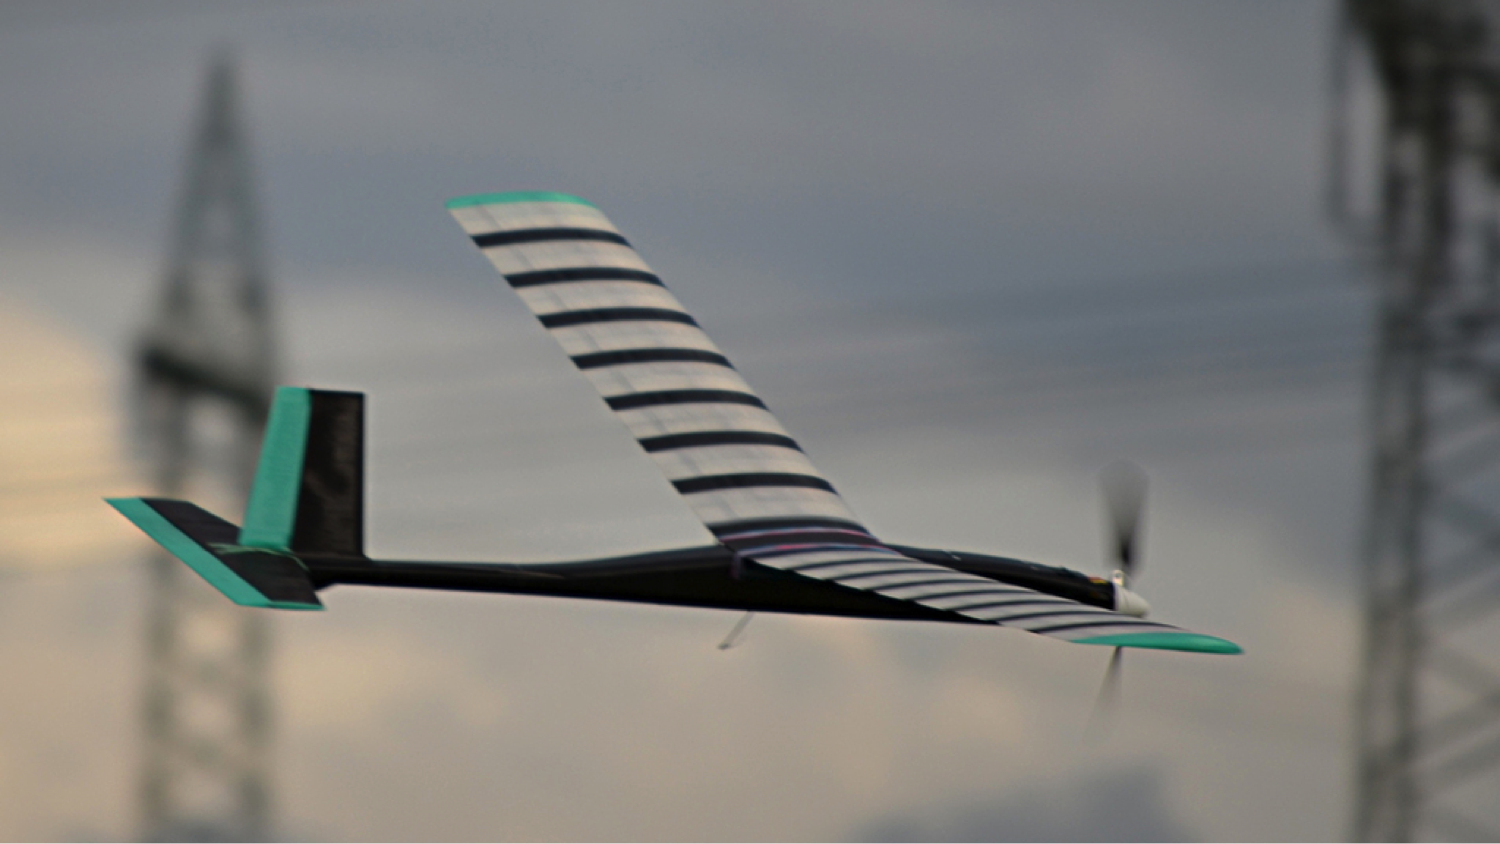
\includegraphics[width=\textwidth]{01-intro-plane}
    \caption{A self-fabricated model airplane.}
    \source{\url{http://thingiverse-production-new.s3.amazonaws.com/renders/05/d7/e9/e9/88/Take_Off_03_preview_featured.jpg} \visited}
    \label{fig:intro-ideas:plane}
  \end{subfigure}
  \begin{subfigure}[b]{\textwidth}
    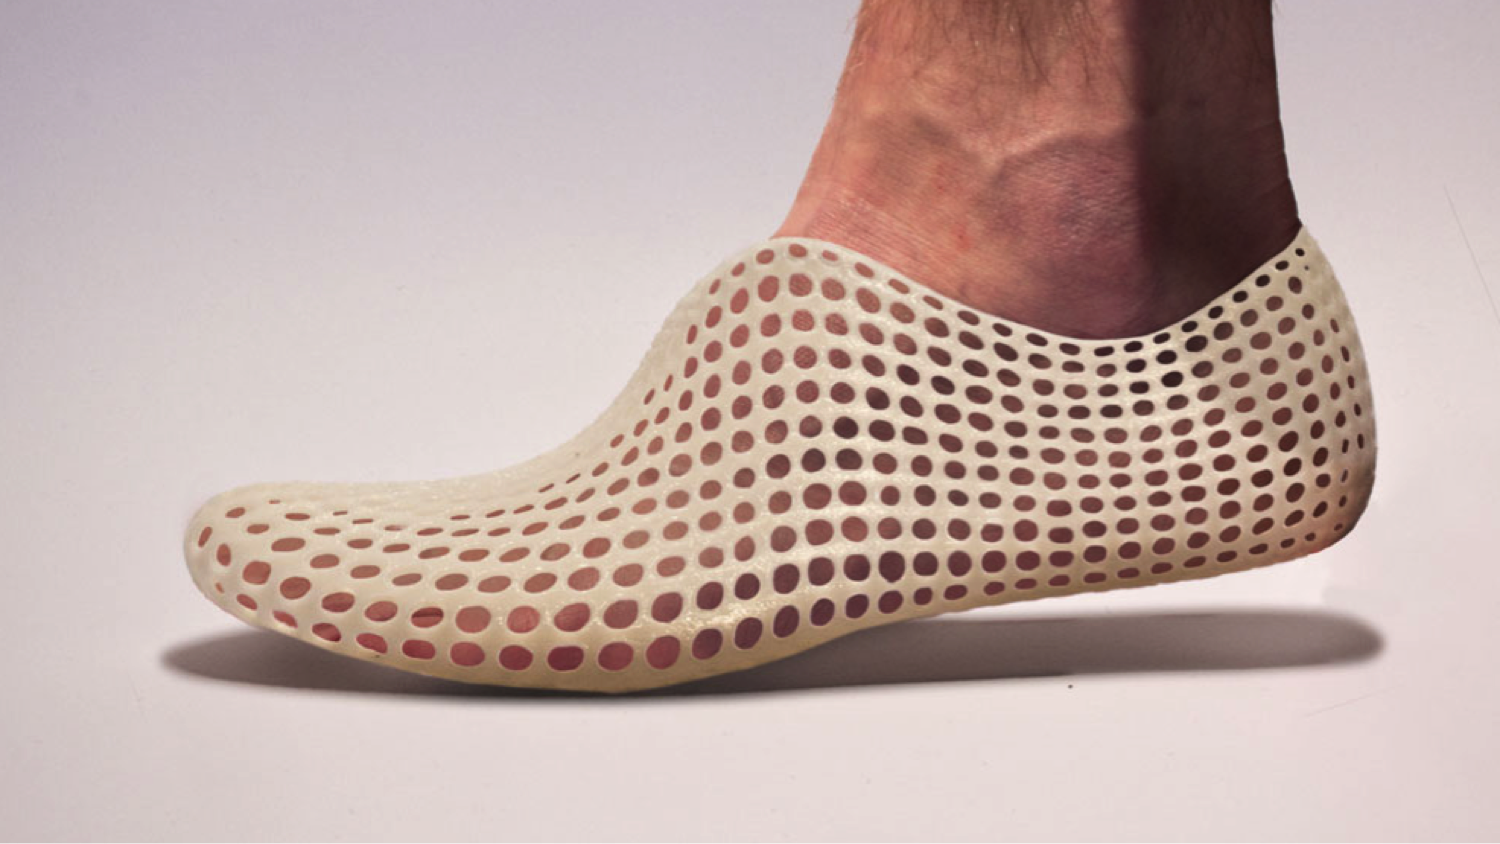
\includegraphics[width=\textwidth]{01-intro-shoe}
    \caption{A shoe with correct fit to its wearer.}
    \source{\copyright Olivier van Herpt, \url{http://oliviervanherpt.com/img/3d-printed-shoes-foot.jpg} \visited}
    \label{fig:intro-ideas:shoe}
  \end{subfigure}
  \begin{subfigure}[c]{\textwidth}
    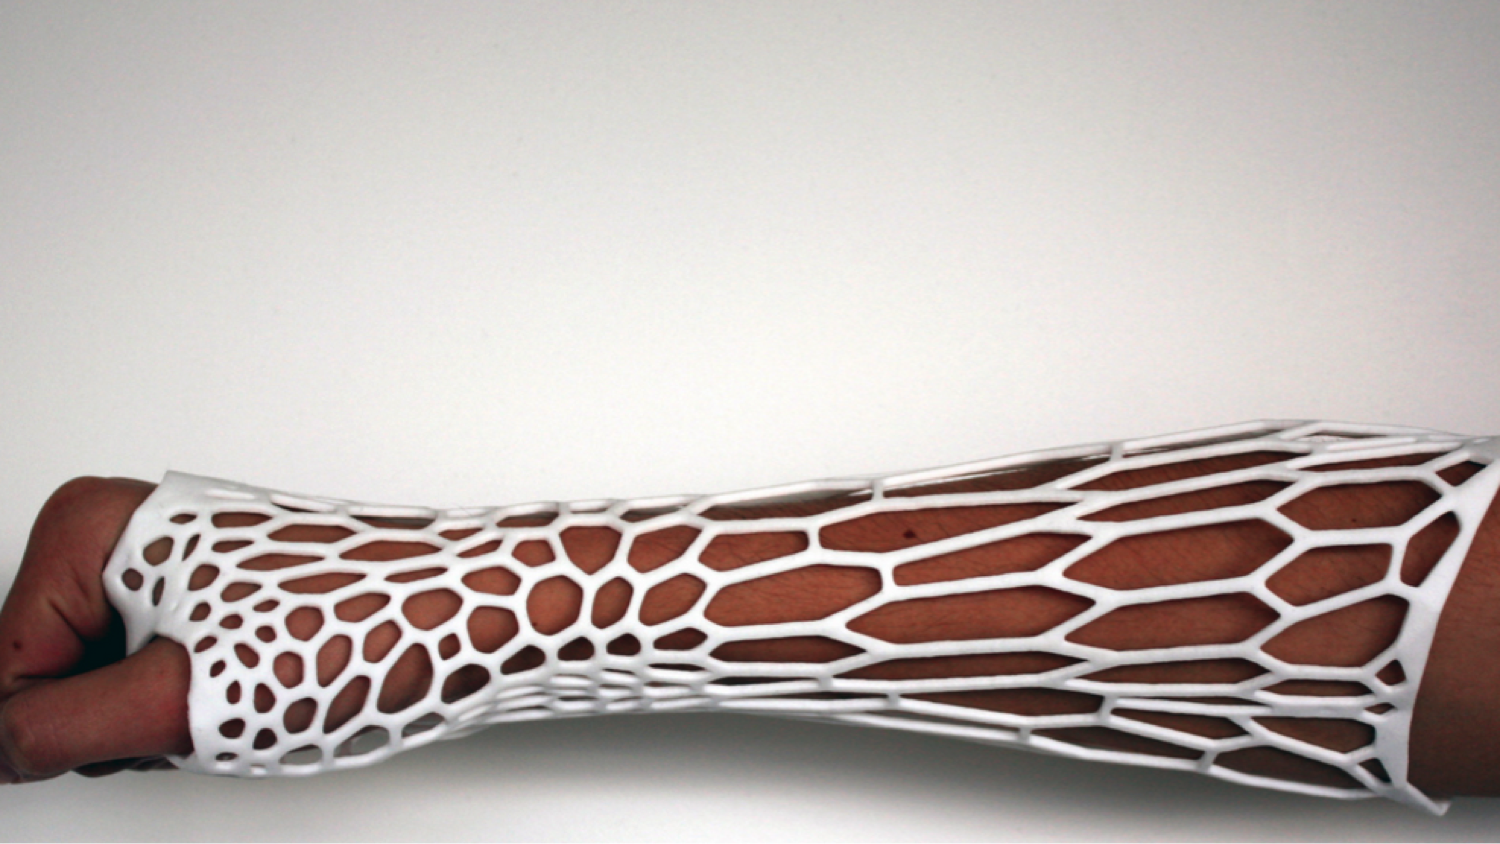
\includegraphics[width=\textwidth]{01-intro-plaster}
    \caption{\name{Cortex}, a fully ventilated plaster.}
    \source{\copyright Jake Evill, \url{http://www.evilldesign.com/image/41499/2000x0-5/p18qh3vpntsq91sg21a261dr114dc6.jpg} \visited}
    \label{fig:intro-ideas:plaster}
  \end{subfigure}
  \caption{With fabrication machines, broad ideas come to life.}
  \label{fig:intro-ideas}
\end{figure}

Before, it was hard to shape these ideas into a physical reality. But
the way ideas are turned into reality is changing. Today machines
exist that, connected to a computer, will take over the fabrication of
objects. Users of fabrication machines can focus on ideas
instead of requiring and acquiring additional skills to actually
fabricate.

% one of theses machines => 3d printer
% market -> growing, machines more and more affordable
% layerwise plastik materials, free forms, easy to use -> button click -> object out.
% but: limitations -> slow, material (lose structure/ beauty)

Such a fabrication machine is a 3D printer. 3D printing is an emerging
technology spreading across the consumer market. According to
\name{Wohlers Associates}, in the year 2015 the 3D printing market was
worth 6.5 billion USD. Their prognosis estimates a roughly 300\%
growth in the next five years \cite{wohlers-market}. With 3D printers
literally any user can produce any free-form object with a button
press. A common technique in 3D printing is fused deposition modeling
(FDM). With the FDM technique
thermoplastic material is heated and then pressed through a nozzle,
mounted on a print head. Material is extruded layer by layer  to
create 3D~objects \cite{fdm}.

Though 3D printing brings a substantial progress to the
field of fabrication, it shows two flaws: 3D printing is
slow, and it is limited in its materials. Even small models
need a couple of hours to be printed. The miniature bird
house (3.5x3.5x5.5cm) in Figure~\ref{fig:intro-bird-house}
printed for three hours\footnote{Printed with the
  \name{Ultimaker~2+},
  \url{https://ultimaker.com/en/products/ultimaker-2-plus}}.
In its original dimensions (20x20x30cm) it requires about
two days of printing time\footnote{Estimated with the
  \name{Cura~2} 3D~printer software,
  \url{https://ultimaker.com/en/products/cura-software}}.
The FDM technique requires material to be extruded through a
nozzle. Thus the material is melted and loses its original
structure and characteristics, like aesthetics or haptics.

\begin{figure}[ht]
  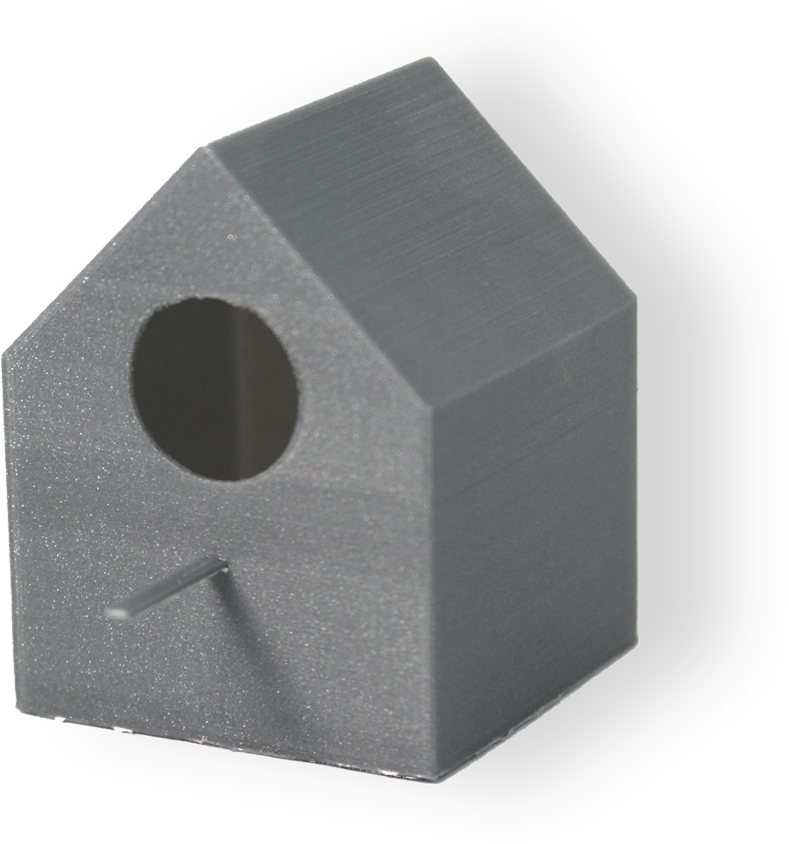
\includegraphics[width=0.6\textwidth]{01-intro-bird-house}
  \caption{A 3D~printed bird house.}
  \label{fig:intro-bird-house}
\end{figure}


% other machine, our target machine -> laser cutter
% cutting materials from a cut plan (typically svg file)
% 2d shapes/ plates
% assembled to objects
% materials like wood, acryllic, textiles, metal or stone
% laser cutter -> low-fi fabrications
% faster than printer
% market laser cutters is coming

% you
% can build 3d things from the laser cutter as well. though not
% freeform, but it is possible iterating on functional objects -> drone
% original materials can be used -> designer glasses but 2 challenges:

Another fabrication machine is the laser cutter, shown in
Figure~\ref{fig:intro-laser:machine}. A laser traces the
outlines of a planar cutting plan, producing plates which
are cut out from flat materials
(Figure~\ref{fig:intro-laser:cut}). Such materials are wood
or acrylic. High-performance devices can cut textile,
metal, and stone. The cutting process requires very short
time, compared to the printing time of a 3D~printer.
Figure~\ref{fig:intro-laser:assembly1} and
Figure~\ref{fig:intro-laser:assembly2} show how the cut-out
plates are assembled to a 3D~object. The entire fabrication
is completed in several minutes.


\begin{figure}[!ht]
  \centering
  \begin{subfigure}[a]{0.49\textwidth}
    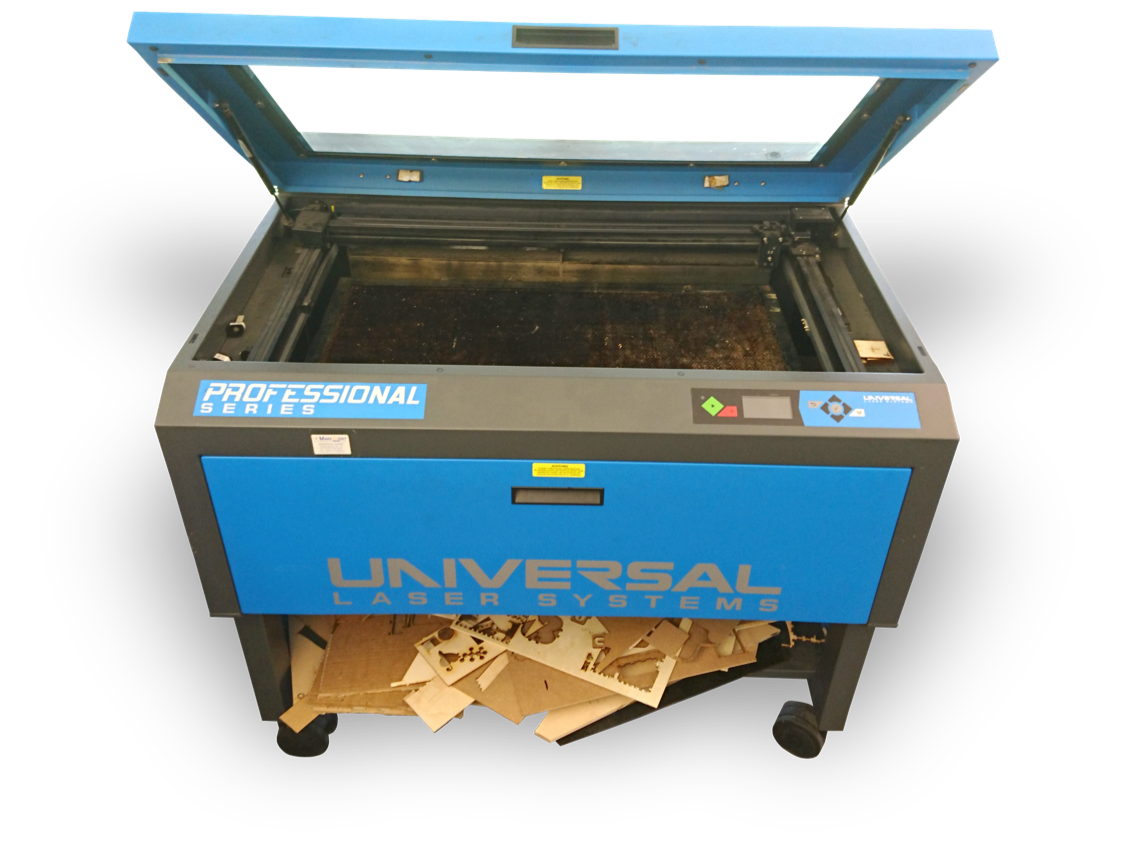
\includegraphics[width=\textwidth]{01-intro-laser-machine}
    \caption{A laser cutter.}
    \label{fig:intro-laser:machine}
  \end{subfigure}
  \begin{subfigure}[b]{0.49\textwidth}
    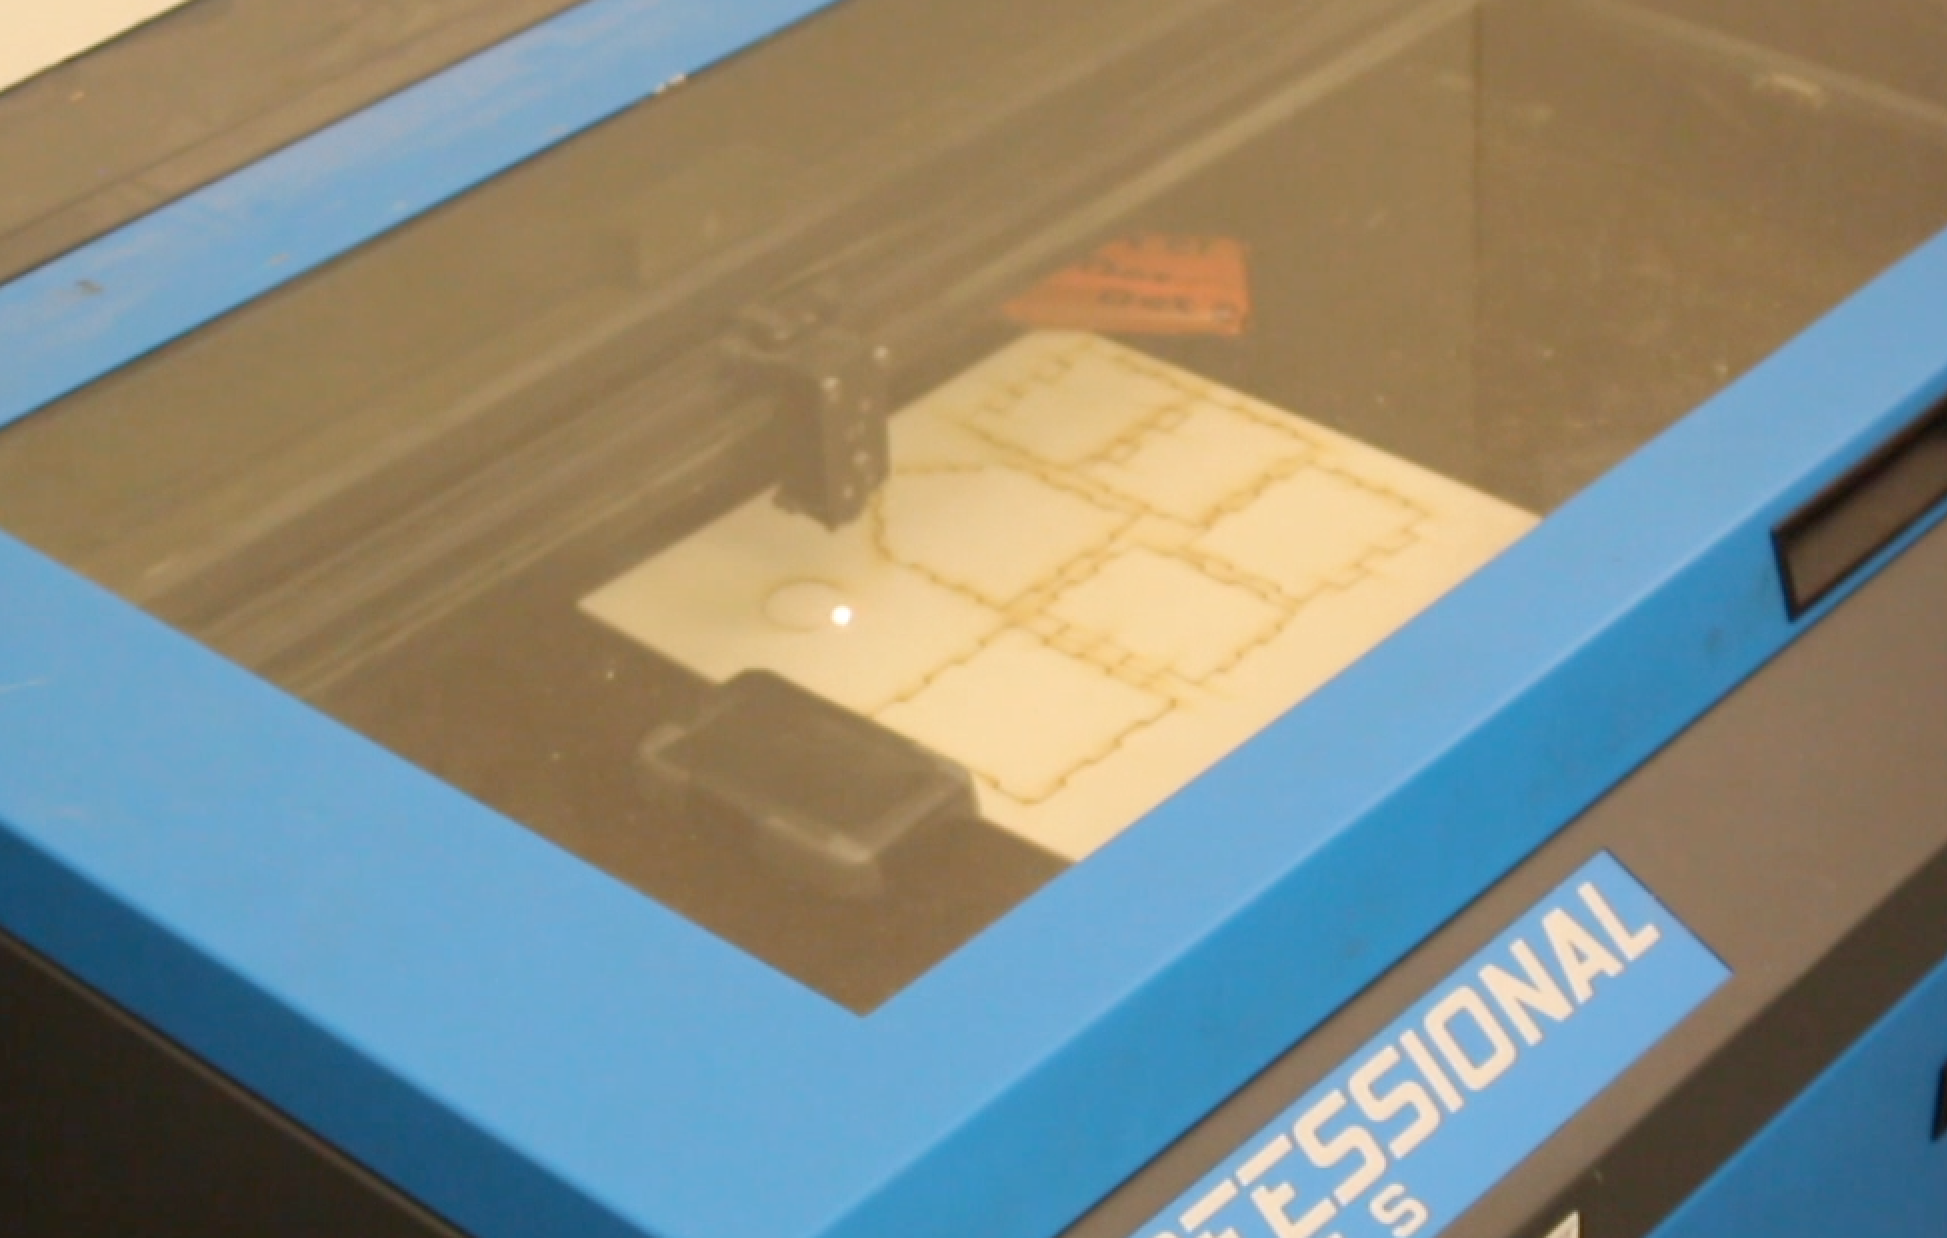
\includegraphics[width=\textwidth]{01-intro-laser-cut}
    \caption{The laser cuts plates from wood.}
    \label{fig:intro-laser:cut}
  \end{subfigure}
  \begin{subfigure}[c]{0.49\textwidth}
    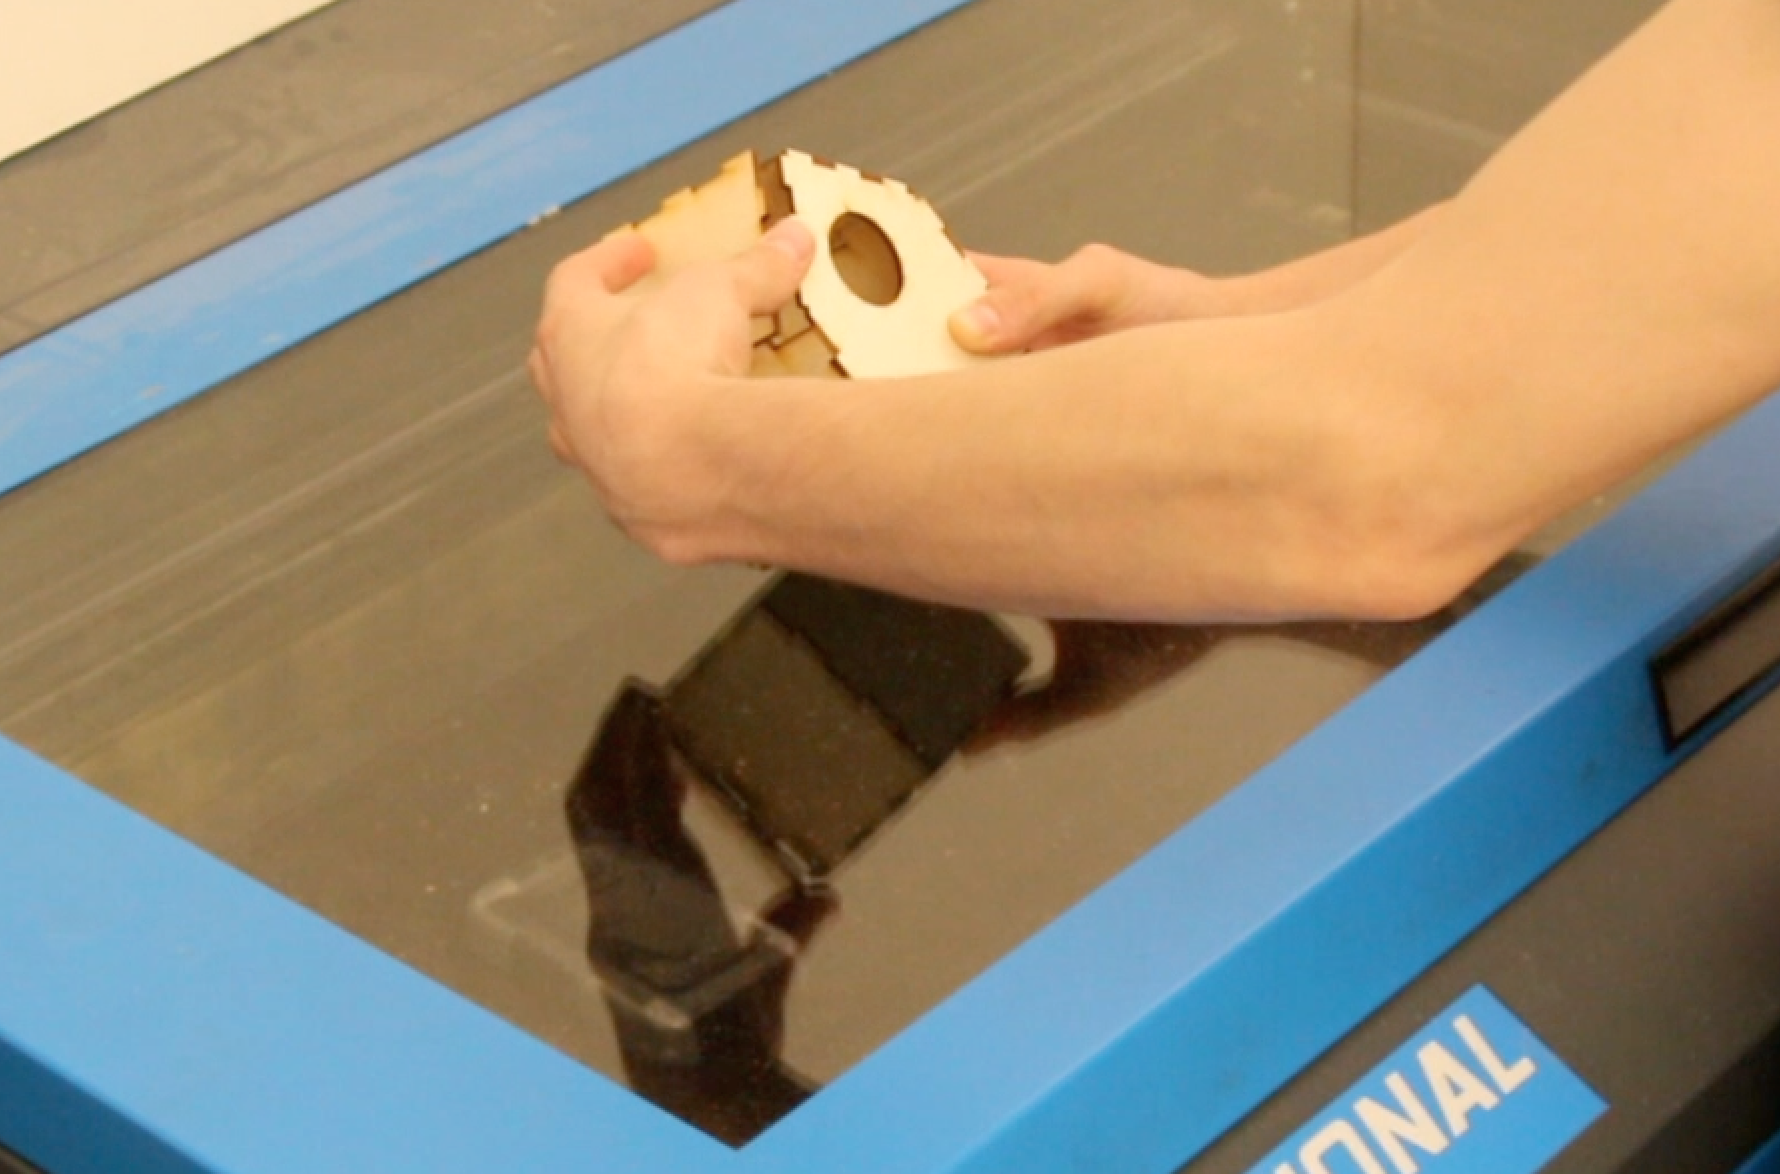
\includegraphics[width=\textwidth]{01-intro-laser-assembly1}
    \caption{Plates are assembled into a 3D~object. }
    \label{fig:intro-laser:assembly1}
  \end{subfigure}
  \begin{subfigure}[d]{0.49\textwidth}
    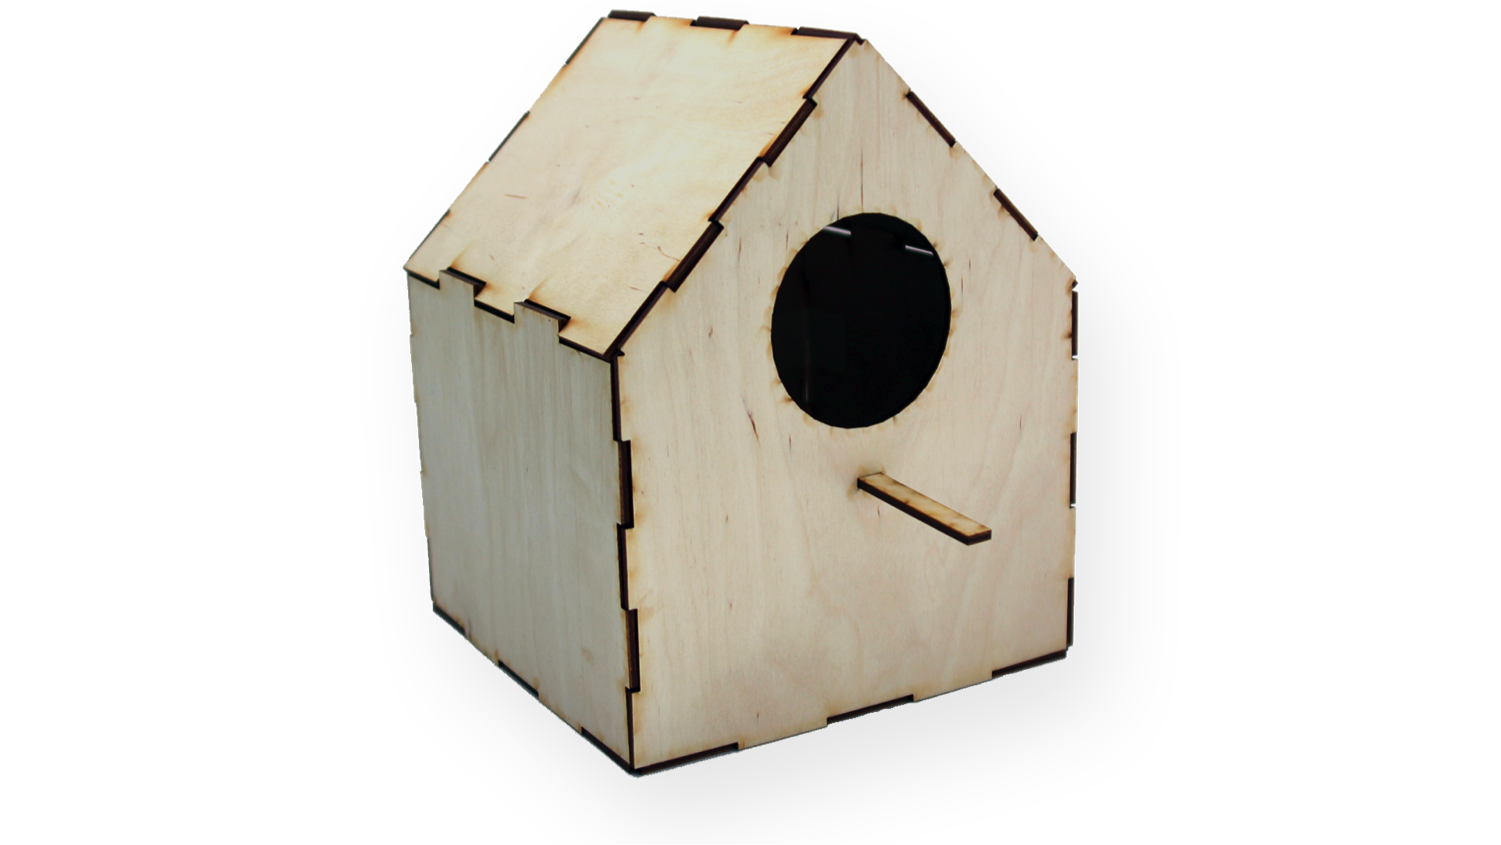
\includegraphics[width=\textwidth]{01-intro-laser-assembly2}
    \caption{The wooden bird house is connected with finger
      joints.}
    \label{fig:intro-laser:assembly2}
  \end{subfigure}
  \caption{Fabrication steps for building a bird house with
    a laser cutter.}
  \label{fig:intro-laser}
\end{figure}

With a laser cutter low-fidelity functional objects are
fabricated. Low-fidelity means producing functional objects
that fulfill their purpose, but lack the amount of detail a
full-fledged product would have. If there is a minor
relevance to structural details of the designed object, the
laser cutter is the perfect choice. Using a laser cutter for
low-fidelity objects will increase the overall efficiency of
the fabrication process. A user can iterate on objects
several times a day to achieve better results.
% In comparison to 3D printing, we can use the time more
% efficiently.
Such a functional object could be a quadcopter produced from
wood, as shown in Figure~\ref{fig:intro-quadcopter}.

\begin{figure}
  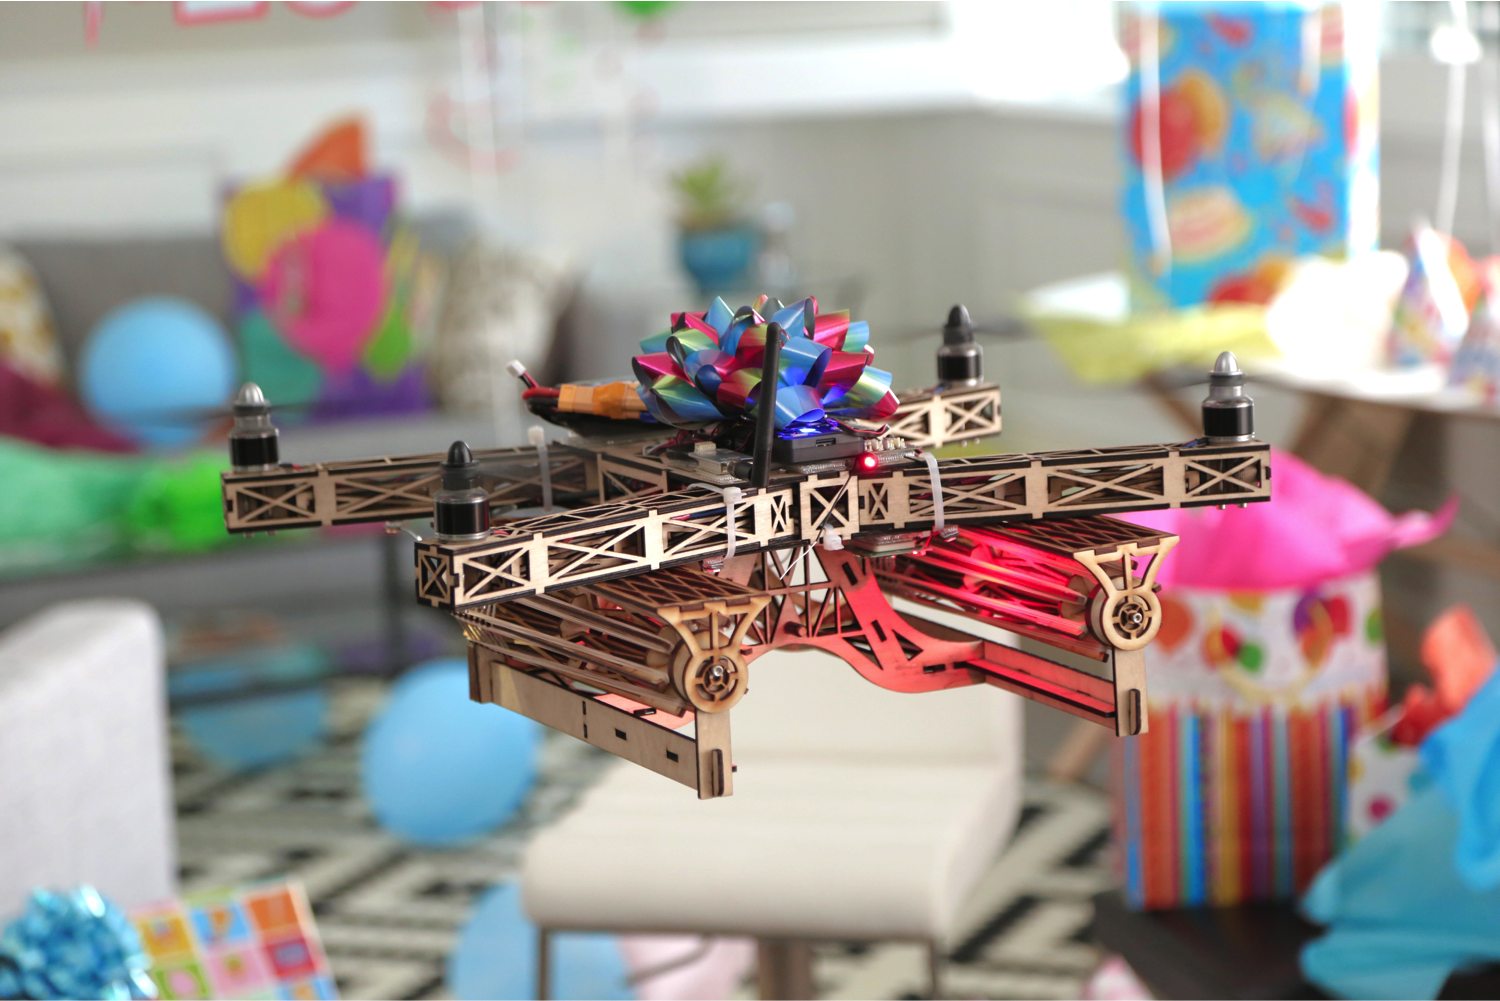
\includegraphics[width=\textwidth]{01-intro-quadcopter}
  \caption{A laser cutted quadcopter.}
  \source{\url{http://wedreamabout.com/wp-content/uploads/2016/01/drone-plywood-mixedbg-2.jpg
    } \visited}
  \label{fig:intro-quadcopter}
\end{figure}

With a laser cutter users can design objects with decorative
aspects as well (Figure~\ref{fig:intro-glasses}).
% The laser cutter preserves the original structure of the
% used materials.
The fabricated object benefits from the original
characteristics of the material.

\begin{figure}
  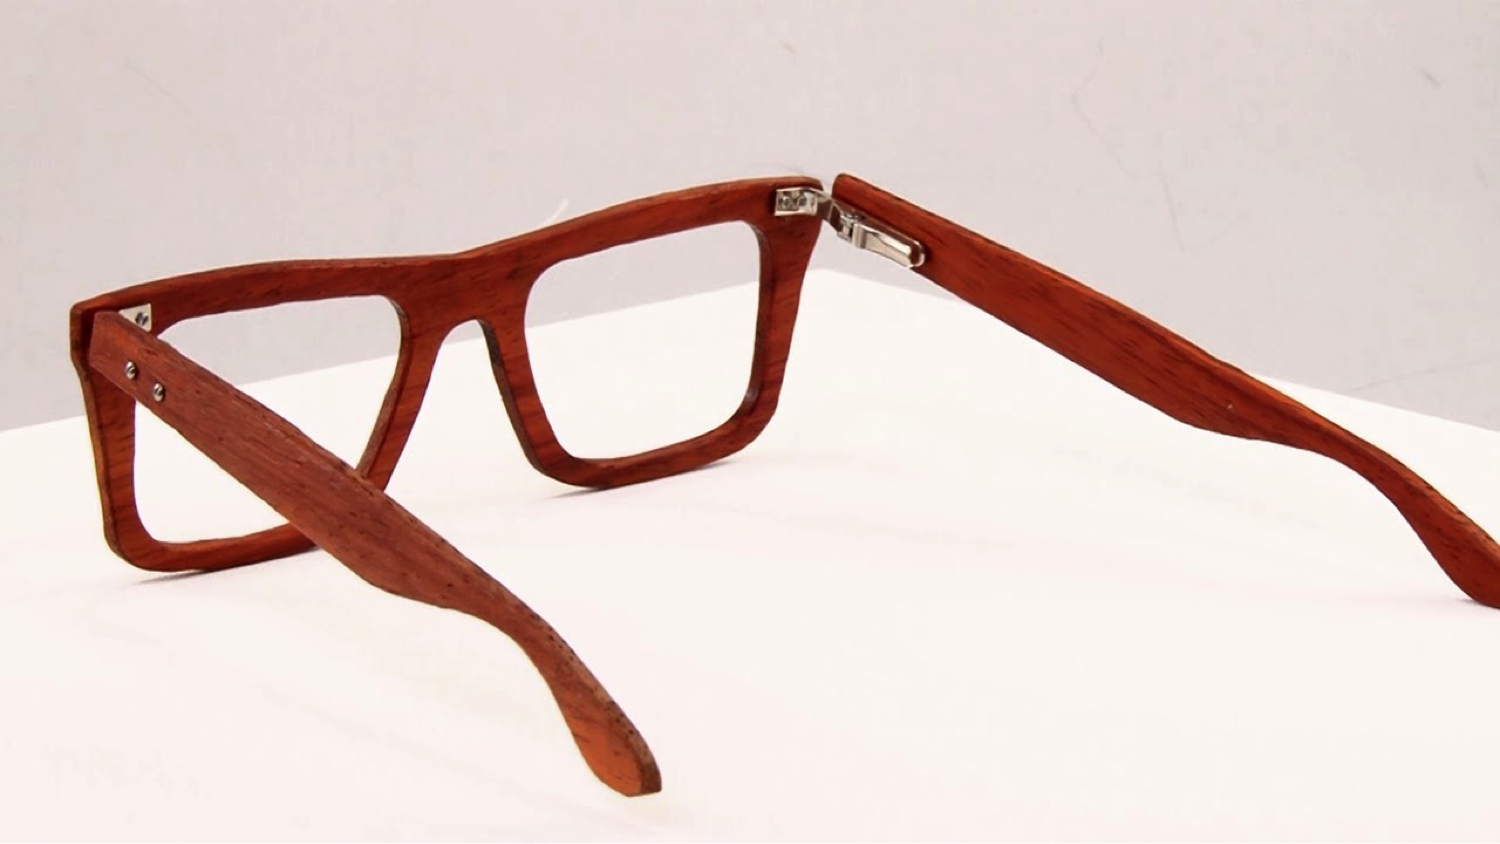
\includegraphics[width=\textwidth]{01-intro-glasses}
  \caption{Wooden designer glasses built with a laser cutter.}
  \source{\url{https://i.ytimg.com/vi/q0dDhesoC08/maxresdefault.jpg} \visited}
  \label{fig:intro-glasses}
\end{figure}

% need to assemble. spatial orientation. need to know where plates from the cutting plan will resemble on final model.
% need knowledge about materials. knowledge a carpenter or craftsman has. fingerjoints for example
% manual drafting of cutting plans for large objects -> difficult
% each connection must be placed exactly, on millimeter, others plates stuck or fall apart

When creating 3D~objects with a laser cutter, users face two
challenges: They need a vast amount of spatial orientation
and craft men's knowledge about the used materials. The
final object has to be assembled from the cut-out plates.
The user has to know where the plates will resemble on the
object in 3D space. Then, the user has to attach the plates
to each other. In the case of wooden plates this would
require knowledge about carpentry. In
Figure~\ref{fig:intro-laser:assembly2} we combined the
plates of a bird house with finger joints. When creating
cutting plans manually for larger objects, detailed work is
required. All connections have to be positioned perfectly.
Otherwise the plates stuck or fall apart during assembly.

% we aim to make 3d model fabrication with laser cutter easy. using its pros in time, material. improving the creation of cut plans
% we present software system platener
% similar intuitive approach as with 3d printing. start from 3d model. user knows how results will look lik.
% our software converts 3d model to a suitable cutting plan.
% analyzes geometries -> approximating a model with plates (different techniques we elaborate on in this thesis)
% putting plates together (software knows which materials -> allowing to place finger joints calibrated for the laser cutting, allowing bends).

In this thesis, we present a solution which enables every
user to produce three dimensional objects with a laser
cutter. We produce cutting plans from {\threedmodel}s
automatically. We improve the creation process of cutting
plans, so that users do not require any additional skills.
Similar to 3D~printing we begin the fabrication process with
a 3D~model.
% Every user can imagine from the model, how the final
% object will look like.
Our software system {\platener} converts the 3D~model to a
2D cutting plan. {\platener} analyzes the geometries and
approximates the model with plates. Users are not required
to map the 2D~cutting plan into 3D~space manually. The
system is aware of common materials used with a laser
cutter. The software generates connections between the
plates. All connections are calibrated, meaning the plates
hold together without using any glue or other means of
attachment. With our software users fabricate 3D~models
easily while benefiting from the working speed of a laser
cutter and free choice of materials.

% in this thesis we talk about:

% architecure
% data structures
% approximation of high-res models
% plate finding
% plate joining
% advanced analysis and conversion technique (future work)

We present our system architecture in
Chapter~\ref{ch:architecture} and give an overview of the
most important data structures in
Chapter~\ref{ch:processingPipeline}. From
Chapter~\ref{ch:approximation} to Chapter~\ref{ch:curves} we
explain the conversion process of 3D~models to 2D~cutting
plans.

\section{Related Work}
\label{sec:related-work}

\paragraph{{\platener}} \citeauthor{master-thesis} did the groundwork
for this thesis. Their work introduced the concept of converting
3D~models to laser cuttable {\svgfile}s as a low-fidelity fabrication
technique. Our work improves the introduced methods, while we focused
on building a user-centered conversion service.

\note{how to keep previous and now platener apart?}
\paragraph{{\brickify}} \citeauthor{bachelor-thesis} present
a low-fidelity fabrication approach using 3D~printers and
{\lego} bricks. Similar to {\platener} they
use a 3D~editor to convert input models. The conversions
result in hybrid models consisting of printed material and
bricks. They improve fabrication time noticeably. They built
a user-oriented web service using WebGL. The implementation
presented in this thesis is based on the implementation of
{\brickify}. {\brickify} is grounded on previous work by
\citeauthor{fabrickation}.

\note{add bib for fabrickation}

\paragraph{LaserOrigami} \citeauthor{laserorigami} present a
low-fidelity prototyping system for creating 3D~models with laser
cutters. Though they have the same goal as {\platener}, they use a
different approach. LaserOrigami cuts and folds the resulting
3D~object from a single piece of acrylic material.
\citeauthor{laserorigami} provide an editor for cutting plans which
incorporates the additional laser cutter instructions for folding. The
objects produced by {\platener} need a manual assembly step. In return
{\platener} allows fabricating objects from a 3D~template.

\note{add bib for laser origami}

\paragraph{SketchChair} With the software SketchChair novice users can
design and fabricate their own chair using a laser cutter. Similar to
{\platener} \citeauthor{sketchchair} provide a system to produce
cutting plans for functional objects from 3D~models. These 3D~models
are generated from two dimensional sketches which are drafted in an
editor. In contrast to SketchChair, {\platener} attempts to convert
any given 3D~model into a laser cuttable template.

\note{add bib for sketchchair}

\paragraph{123Make} Autodesk\footnote{\url{http://www.autodesk.de/}}
ships a 3D~editor which converts 3D~models into slices. These slices
can be cut with a laser cutter and stacked onto each other to
approximate the original model. This method solely provides an
approximation of the external shape of the object. Though {\platener}
provides this technique as well, we focus on maintaining the
functional aspect of the input model.

\note{some source for 123make}

\end{document}

%%% Local Variables:
%%% mode: latex
%%% TeX-master: "../ClassicThesis"
%%% TeX-command-extra-options: "-shell-escape"
%%% End:
